\section{Reducing Linearizability of Priority Queues into State Reachability}
\label{sec:co-regular of extended priority queues}

In this section, we divide checking linearizability w.r.t $\seqPQ$ into checking linearizablity w.r.t $\Gamma\mathsf{\text{-}Seq}(s,\alpha)$, each of which can be done in polynomial-time. Due to data-independence, violations to each $\Gamma\mathsf{\text{-}Seq}(s,\alpha)$ can be captured by register automata. This reduces checking linearizability w.r.t $\seqPQ$ into state reachability problem.  



\subsection{Co-Regular}
\label{subsec:definition of co-regular} 

Let $\Gamma\mathsf{\text{-}Condition}(e)$ be $\mathsf{HasEmptyRemoves}(e)$, $\neg \mathsf{HasEmptyRemoves}(e) \wedge \mathsf{HasUnmatchedMaxPriority}(e)$, and $\mathsf{HasMatchedMaxPriority}(e)$, for $\Gamma = \mathsf{EmptyRemove}, \mathsf{UnmatchedMaxPriority}, \mathsf{MatchedMaxPriority}$, respectively. $\textit{Check-PQ-Conc}$ inspires us that, whenever $\Gamma\mathsf{\text{-}Condition}(e)$ holds, there should exist some $\alpha$, such that  $\Gamma\mathsf{\text{-}Conc}(e,\alpha)$ holds. The following lemma states this formally. Let $\textit{proj}(e)$ be the set of projections of $e$ into set of values. When refer to $\textit{proj}(e)$, we implicitly assume that each $\textit{rm}(\textit{empty})$ in $e$ has a ghost argument that is unique.

\begin{restatable}{lemma}{EPQasMultiInMRpriforHistory}
\label{lemma:EPQ as multi in MRpri for history}
Given a data-differentiated execution $e$, $e \sqsubseteq \seqPQ$, if and only if, $\forall e' \in \textit{proj}(e)$, $\Gamma\mathsf{\text{-}Condition}(e) \Rightarrow \Gamma\mathsf{\text{-}Conc}(e,\alpha)$ holds for some $\alpha$
\end{restatable} 

Register automata is a kind of finite automata with registers used to deal with infinite data domain, where register can be assigned values and do simple operations. In this paper we use a restricted kind of register automata, which contains only one register, whose value is obtained once by guessing and never changed. Our register machine contains a register $\textit{reg}$. Its transition labels are $\textit{call}(\textit{put},d,p,g), \textit{ret}(\textit{put},d,p),$ $\textit{call}(\textit{rm},d),\textit{ret}(\textit{rm},d)$, where $d \in \mathbb{D} \cup \{ \textit{empty} \}$, and $g$ and $\top$ are guards. A guard is a predicate chosen from $\{\textit{equalReg},\textit{lesReg},\top \}$, which represents equals the value of $\textit{reg}$, less than the value of $\textit{reg}$, and always holds, respectively. Given an execution $e = \alpha_1 \cdots \alpha_k$ of priority queue, register automata $\mathcal{A}$ accepts $e$, if there exists value $p \in \in \mathbb{D}$ and transitions $q_0 \xrightarrow{\beta_1} q_1 \ldots \xrightarrow{\beta_k} q_k$ of $\mathcal{A}$ from a initial state to a final state, such that for each $i$

\begin{itemize}
\setlength{\itemsep}{0.5pt}
\item[-] If $\alpha_i = \textit{call}(\textit{put},a,p)$, then $\beta_i= \textit{call}(\textit{put},a,p,g)$ and $g(q)$ holds. 

\item[-] Else, $\alpha_i = \beta_i$. 
\end{itemize}

Note that due to data-independence, register automata are used to detect some renamed violations, instead of store and checking directly. 




Let us introduce the notion of co-regular, which reduce checking linearizable w.r.t $\Gamma\mathsf{\text{-}Conc}(e,\alpha)$ into checking set of witness automata.

%\vspace{-6pt}
\begin{definition}\label{def:co-regular of rules of extended priority queues}
Given $R \in \{ \textit{EPQ}_1^{>}, \textit{EPQ}_1^{=}, \textit{EPQ}_2^{>}, \textit{EPQ}_2^{=}, \textit{EPQ}_3 \}$. $R$ is co-regular, if there are a finite set $\textit{Auts}_{R}$ of witness automata such that, for each data-independence implementation $\mathcal{I}$, we have that

$$\textit{Auts}_{R} \cap \mathcal{I} \neq \emptyset \Leftrightarrow \exists e \in \mathcal{I}_{\neq},e' \in \textit{proj}(e), R \in last(e') \wedge e' \not\sqsubseteq \textit{MS}(R)$$

We say that $\textit{EPQ}$ is co-regular, if all five candidates of $R$ are co-regular.
\end{definition}

We simply the proof of co-regular of $\textit{EPQ}$ in two side. The first side uses the results in \cite{Bouajjani:2015} to ensure FIFO (first in first out) property of each single-priority projections. A execution where only items of one priority is putted is called a single-priority execution. It is obvious that each single-priority projection of sequences in $\textit{EPQ}$ satisfy FIFO property. Let $\textit{transToQueue}(e)$ be an execution generated from $e$ by transforming $\textit{put}$ and $\textit{rm}$ into $\textit{enq}$ and $\textit{deq}$, respectively, and then discarding priorities. In Appendix \ref{sec:appendix proof and definition in section definition of co-regular}, according to the result of queue in \cite{Bouajjani:2015}, we construct a set $\textit{Auts}_{\textit{sinPri}}$ of witness automata, and shows that they are enough to ensure that for each data-differentiated executions, each of its single-priority projection without $\textit{rm}(\textit{empty})$ to have ``FIFO'' property, as shown by the following lemma.

\begin{restatable}{lemma}{AutoForEPQwithSignlePri}
\label{lemma:automata for extended priority queue with single priority}

Given a data-independent implementations $\mathcal{I}$ of extended priority queue, $\mathcal{I} \cap \textit{Auts}_{\textit{sinPri}} \neq \emptyset$, if and only if there exists $e \in \mathcal{I}_{\neq}$, $e' \in \textit{proj}(e)$, such that $e'$ is single-priority  without $\textit{rm}(\textit{empty})$, and $\textit{transToQueue}(e')$ does not linearizable to queue.
\end{restatable}

According to Lemma \ref{lemma:automata for extended priority queue with single priority}, from now on, it is safe to assume that, for each data-differentiated execution without $\textit{rm}(\textit{empty})$, any of its single-priority projection has ``FIFO'' property. For example, $\textit{rm}(a)$ never happens before $\textit{put}(a,\_)$ for each $a$.

The second side is to ignore the incomparable priorities. Given a data-differentiated execution $e$, we say that $e$ is a $\textit{pri}$-execution, if $\textit{pri}$ is the maximal priority of $e$, and $\textit{pri}$ is larger than or equal to the priority of all other items of $e$. Given a data-differentiated execution $e$ and assume that $\textit{pri}$ is one of the maximal priority of $e$, let $\textit{pri-Exec}(e)$ be an execution obtained from $e$ by erasing all operations of items whose priority are incomparable with $\textit{pri}$. The following lemma states that when checking co-regular of $\textit{EPQ}$, it is safe to consider $\textit{pri}$-executions. We can see that $\textit{last}(e')$ contains at most one element for $\textit{pri}$-execution $e'$.

\begin{restatable}{lemma}{priExecutionIsEnough}
\label{lemma:pri execution is enough}
Given a data-differentiated execution $e$ and $R = \textit{EPQ}_1^{>}$ (resp., $R = \textit{EPQ}_1^{=}$, $R=\textit{EPQ}_2^{>}$, or $R = \textit{EPQ}_2^{=}$). $e \sqsubseteq \textit{MS}(R)$ with witness $x$, if and only if $\textit{pri-Exec}(e) \sqsubseteq \textit{MS}(R)$ with witness $x$, where $\textit{pri}$ is the priority of $x$. %for each $\textit{pri}$ that is (1) maximal in $e$ and (2) items of $\textit{pri}$ are only one pair of matched $\textit{put}$ in $e$ (resp., more than one pair of matched $\textit{put}$, unmatched $\textit{put}$, or unmatched $\textit{put}$ and matched $\textit{put}$).
\end{restatable}



\subsection{Co-Regular of $\textit{EPQ}_1^{>}$}
\label{subsec:co-regular of EPQ1Lar}

In this subsection, we briefly introduce the idea for proving co-regular of $\textit{PQ}_1^{>}$. The proof of this subsection can be found in Appendix \ref{sec:appendix proof and definition in section co-regular of EPQ1Lar}. The notion of left-right constraint used for extended priority queue is inspired by left-right constraint of queue \cite{Bouajjani:2015}.

Given a data-differentiated $\_$-execution $e$ such that $\textit{last}(e) = \textit{EPQ}_1^{>}$, Lemma \ref{lemma:automata for extended priority queue with single priority} is not enough for ensuring that $e \sqsubseteq \textit{MS}(\textit{EPQ}_1^{>})$. This is because that it is possible that $e \not\sqsubseteq \textit{MS}(\textit{EPQ}_1^{>})$ because of interaction between actions of multiple priorities. One such example is shown in \figurename~\ref{fig:introduce gap for EPQ1Lar}. We call the time interval from $\textit{ret}(\textit{put},x)$ to $\textit{cal}(rm,x)$, or from $\textit{ret}(\textit{put},x)$ when $\textit{cal}(rm,x)$ does not exist, the interval of item $x$. In \figurename~\ref{fig:introduce gap for EPQ1Lar}, we draw the interval of each item by dashed line. Here we assume that $p_1 <_{\mathbb{P}} p_4$, $p_2 <_{\mathbb{P}} p_4$ and $p_3 <_{\mathbb{P}} p_4$. The reason of $e \not\sqsubseteq \textit{MS}(\textit{PQ}_1^{>})$ is that, each time point from $\textit{cal}(\textit{rm},b)$ to $\textit{ret}(\textit{rm},b)$ is in interval of some item with smaller priority.

\begin{figure}[htbp]
  \centering
  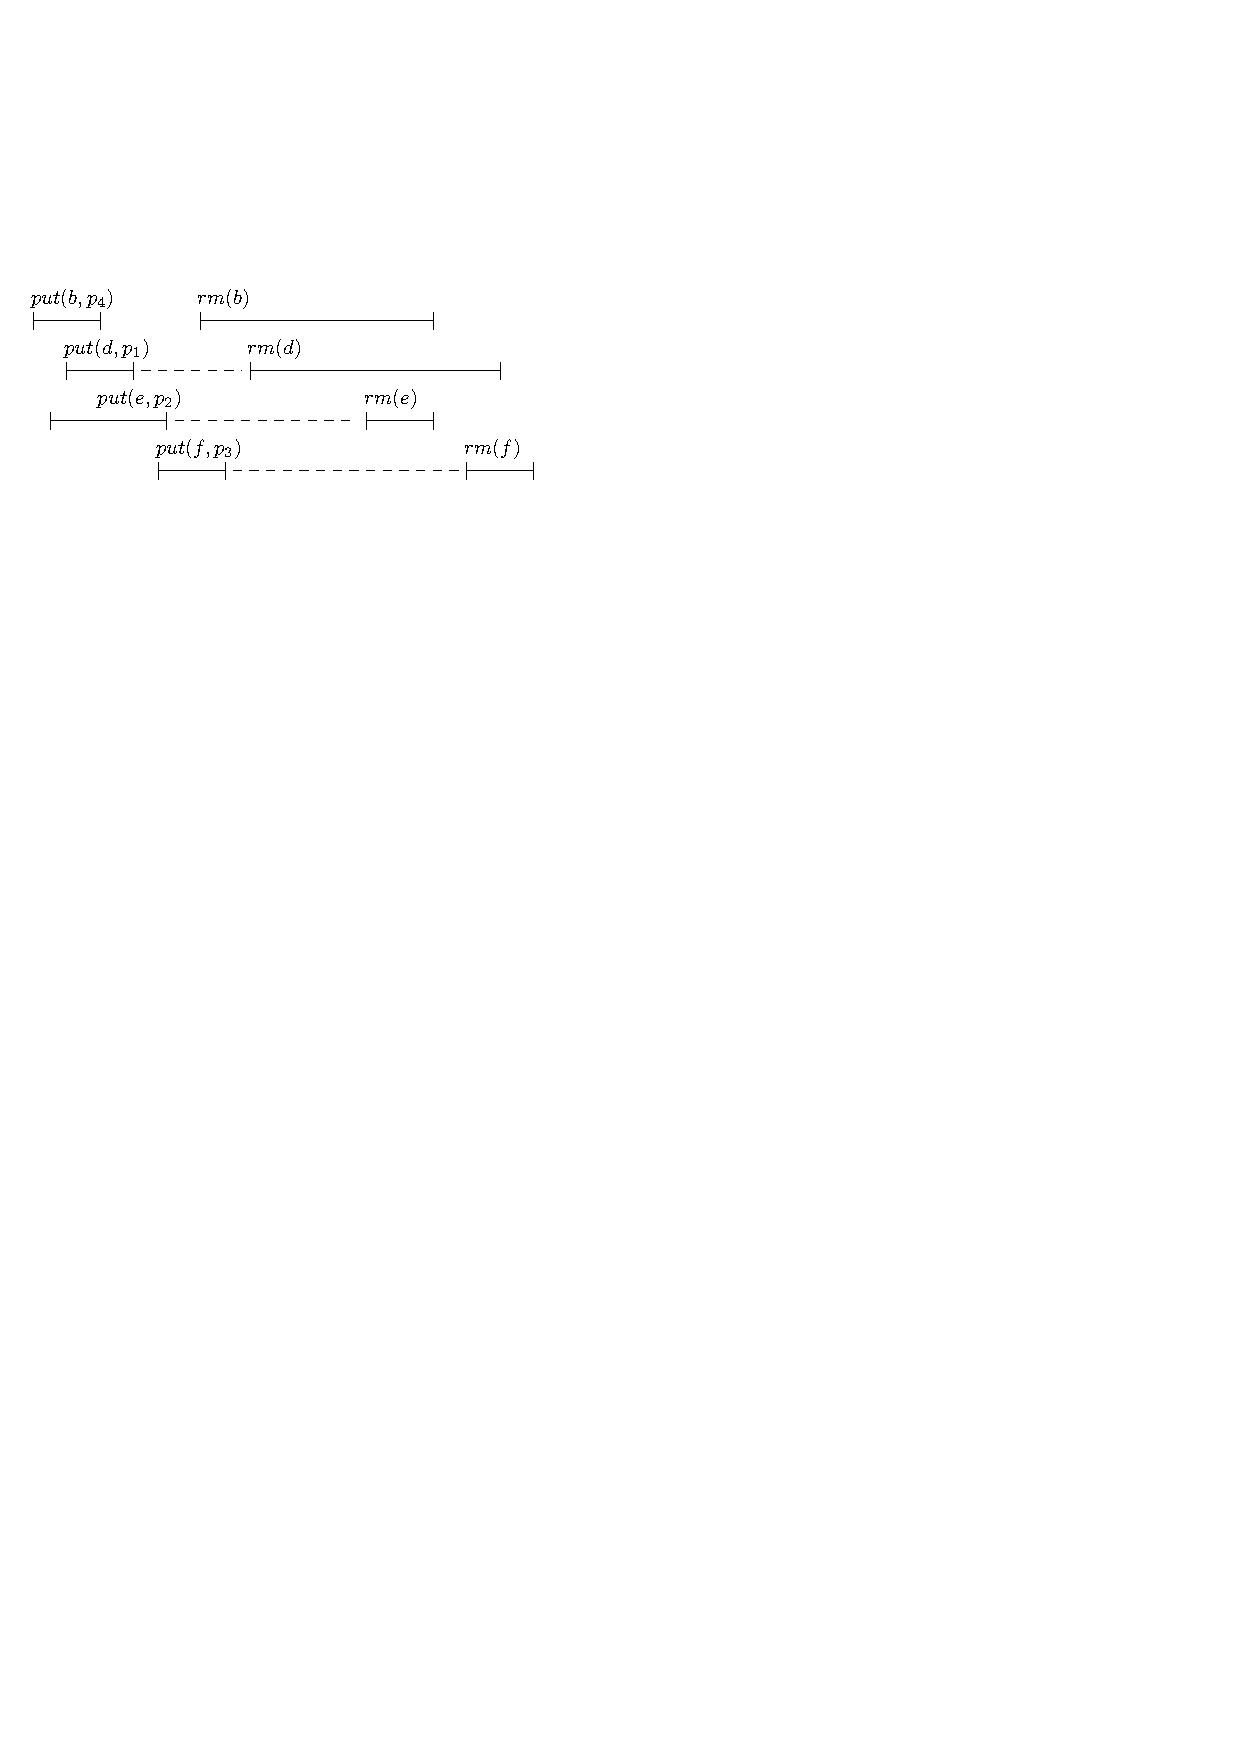
\includegraphics[width=0.4 \textwidth]{figures/PIC-HIS-INTRO-GAP-EPQ1L.pdf}
%\vspace{-10pt}
  \caption{An execution that does not linearizable w.r.t $\textit{MS}(\textit{EPQ}_1^{>})$}
  \label{fig:introduce gap for EPQ1Lar}
\end{figure}

In Appendix \ref{sec:appendix proof and definition in section co-regular of EPQ1Lar}, we introduce the notion of left-right constraint, which is a graph, and the existence of cycle though item with maximal priority in it formally modelled the case in \figurename~\ref{fig:introduce gap for EPQ1Lar}. When there is a cycle $d_1 \rightarrow \ldots \rightarrow d_m \rightarrow x \rightarrow d_1$ through item $x$ with maximal priority in left-right constraint, we say that $x$ is covered by $d_1,\ldots,d_m$ For example, in \figurename~\ref{fig:introduce gap for EPQ1Lar}, $b$ is covered by $f$, $e$ and $d$. We then prove that getting rid of cycle though item with maximal priority in left-right constraint is enough for ensure linearizable w.r.t $\textit{MS}(\textit{EPQ}_1^{>})$, as stated by the following lemma:

\begin{restatable}{lemma}{LinEqualsConstraintforEPQOneLar}
\label{lemma:Lin Equals Constraint for EPQ1Lar}
Given a data-differentiated $\textit{pri}_x$-execution $e$ with $\textit{last}(e) = \textit{EPQ}_1^{>}$. Let $\textit{put}(x,\textit{pri}_x)$ and $\textit{rm}(x)$ be method events of $e$ with maximal priority. Let $G$ be the graph representing the left-right constraint of $\textit{put}(x)$ and $\textit{rm}(x)$. $e \sqsubseteq \textit{MS}(\textit{EPQ}_1^{>})$, if and only if $G$ has no cycle going through $x$.
\end{restatable}

Assume that $x$ is covered by $d_1,\ldots,d_m$, we can safely rename $x$ into $b$, rename $d_1,\ldots,d_m$ into $a$ and rename all other item into $c$ by data-independence. Such execution can be recognized by witness automata, since between the first $\textit{ret}(\textit{put},a,\_)$ and the last $\textit{cal}(\textit{rm},a)$ (if exists), $\textit{ret}(\textit{put},a,\_)$ and $\textit{cal}(\textit{rm},a)$ occurs in pair and there is no need for count. In Appendix \ref{sec:appendix proof and definition in section co-regular of EPQ1Lar}, we construct a set $\textit{Auts}_{\textit{1-lar}}$ of witness automata, and use $\textit{Auts}_{\textit{1-lar}}$ to prove that $\textit{EPQ}_1^{>}$ is co-regular, as stated by the following lemma.

\begin{restatable}{lemma}{EPQOneLarisCoRegular}
\label{lemma:EPQ1Lar is co-regular}
$\textit{EPQ}_1^{>}$ is co-regular.
\end{restatable}




\subsection{Co-Regular of $\textit{EPQ}_1^{=}$}
\label{subsec:co-regular of EPQ1Equal}

In this subsection, we briefly introduce the idea for proving co-regular of $\textit{EPQ}_1^{=}$. The proof of this subsection can be found in Appendix \ref{sec:appendix proof and definition in section co-regular of EPQ1Equal}.

Given a data-differentiated $\_$-execution $e$ such that $\textit{last}(e) = \textit{EPQ}_1^{=}$. Lemma \ref{lemma:automata for extended priority queue with single priority} and $\textit{Auts}_{\textit{1-lar}}$ are sill not enough for ensure that $e \sqsubseteq \textit{MS}(\textit{EPQ}_1^{=})$. This is because that given items $a$ and $b$ with maximal priority, it is possible that all the possible linearization point of $\textit{rm}(b)$ are disabled by $\textit{rm}(b)$. We give an example of such execution $e$ in \figurename~\ref{fig:introduce pb order}. The execution $e$ of \figurename~\ref{fig:introduce pb order} is not linearizable w.r.t $\textit{EPQ}$, even if $h \vert_{p_1}$ and $h \vert_{p_4}$ both does, and either $a$ or $b$ is covered by items with smaller priority. The explanation of $e \not\sqsubseteq \textit{EPQ}$ is as follows: Since $\textit{put}(a,p_4) <_{\textit{hb}} \textit{put}(b,p_4)$, the linearization points of $\textit{rm}(a)$ should before the linearization point of $\textit{rm}(b)$. According to Lemma \ref{lemma:Lin Equals Constraint for EPQ1Lar}, the time intervals identified with dotted lines in \figurename~\ref{fig:introduce pb order} are are possible position to locate the linearization point of $\textit{rm}(b)$. However, each of them is before $\textit{cal}(\textit{rm},a)$.

\begin{figure}[htbp]
  \centering
  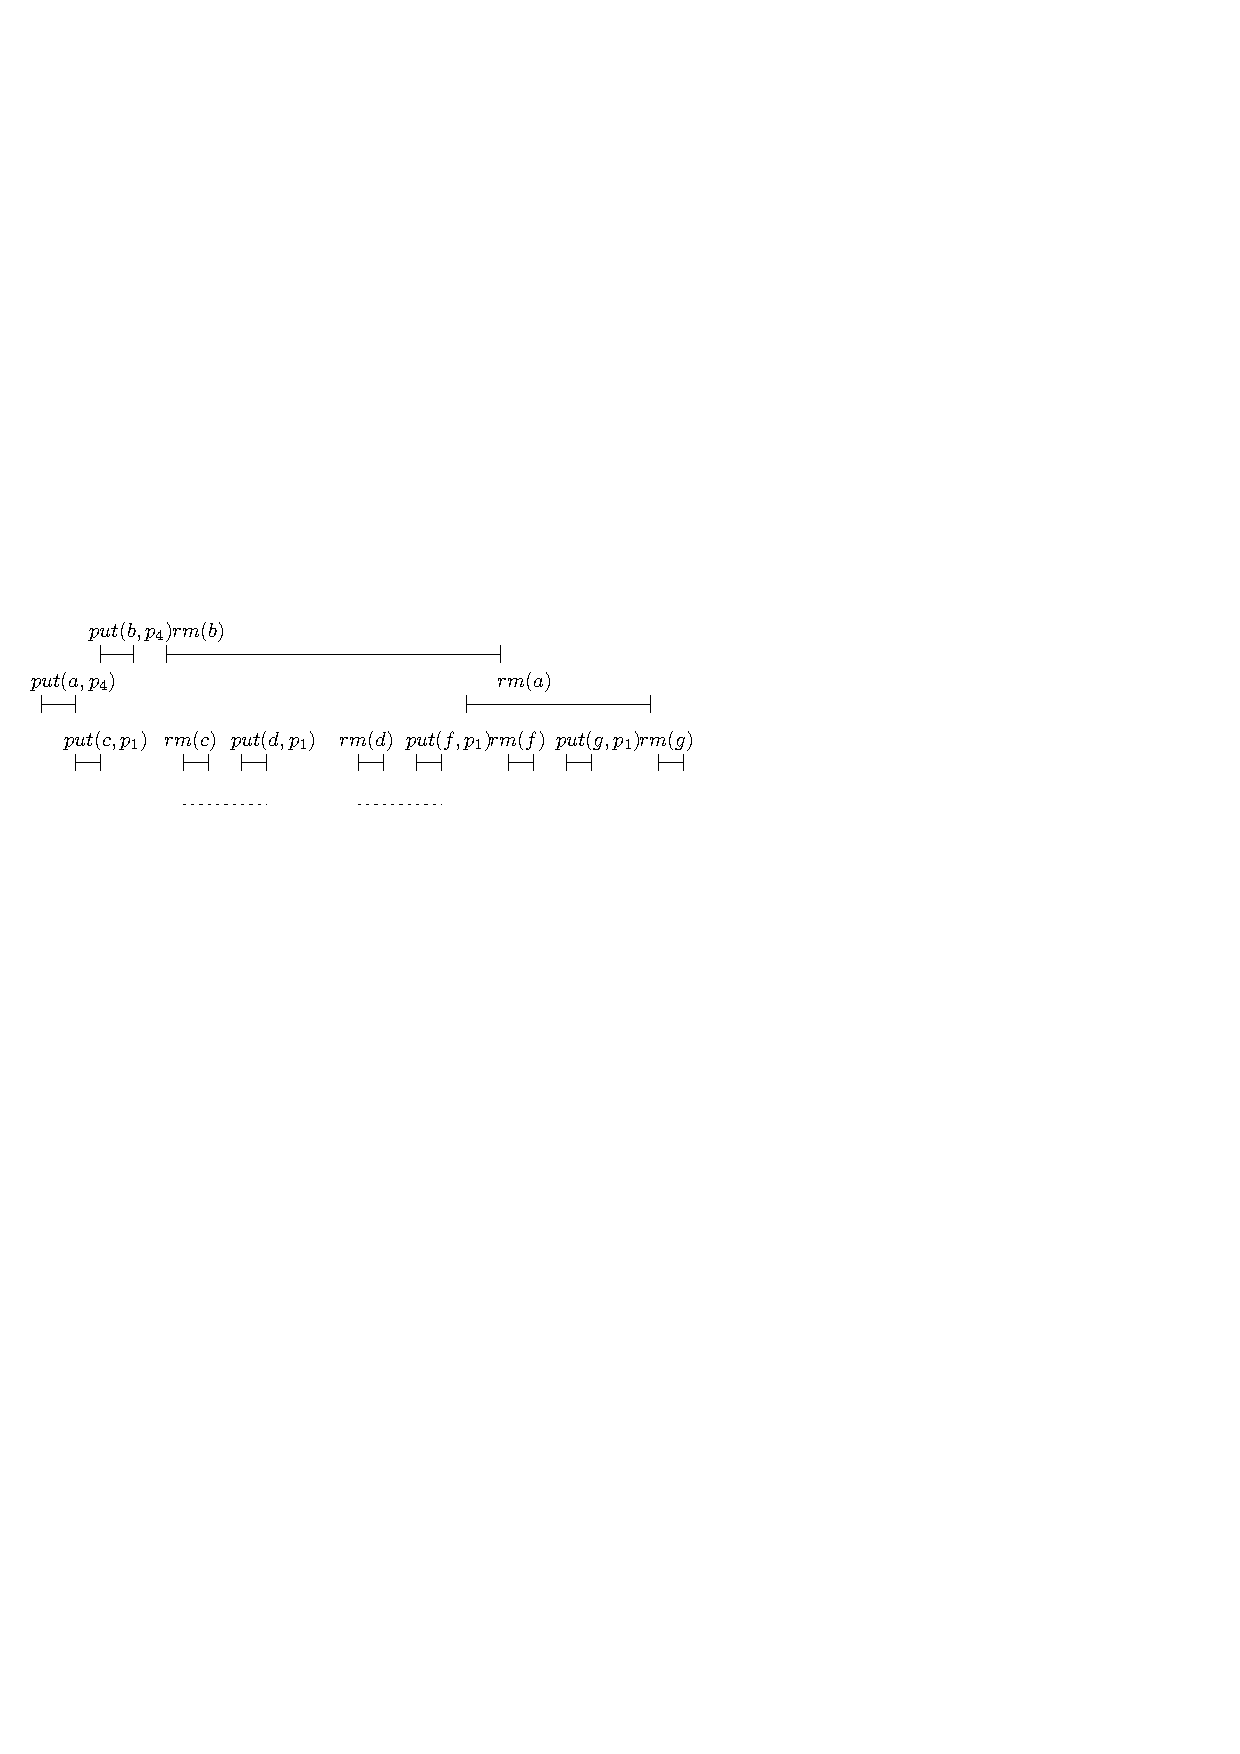
\includegraphics[width=0.6 \textwidth]{figures/PIC-HIS-INTRO-PB-ORDER-EPQ.pdf}
%\vspace{-10pt}
  \caption{An execution that does not linearizable w.r.t $\textit{MS}(\textit{EPQ}_1^{=})$}
  \label{fig:introduce pb order}
\end{figure}

Let us introduce put-before order $<_{\textit{pb}}$ to formally state that ``an item is putted before another item''. Given a data-differentiated $\_$-execution $e$ and two items $a,b$ with maximal priority, $a <_{\textit{pb}} b$, if one of the following cases holds: (1) $\textit{put}(a,\_) <_{\textit{hb}} \textit{put}(b,\_)$, (2) $\textit{rm}(a) <_{\textit{hb}} \textit{rm}(b)$, or (3) $\textit{rm}(a) <_{\textit{hb}} \textit{put}(b,\_)$. Sometimes we use $a <_{\textit{pb}}^A b$, $a <_{\textit{pb}}^B b$ and $a <_{\textit{pb}}^C b$ to explicitly distinguish above three cases. Let $<_{\textit{pb}}^*$ be the transitive closure of $<_{\textit{pb}}$. Intuitively, $a <_{\textit{pb}}^* b$ means that we can infer that $a$ should be putted earlier than $b$ with the help of several other items.

Let us introduce gap-point to formally define the time point in dotted line of \figurename~\ref{fig:introduce pb order}.

\begin{definition}\label{def:gap-point for matched put and rm operations}
Given a data-differentiated $\textit{pri}_x$-execution $e$ and two method events $\textit{put}(x,\textit{pri}_x),\textit{rm}(x)$ of $e$. We say that a time-point $o$ is a gap-point of $x$, if $o$ is after $\textit{call}(\textit{put},x,\textit{pri}_x)$ and $\textit{call}(\textit{rm},x)$, is before $\textit{ret}(\textit{rm},x)$, and is not in interval of any items with smaller priority.
\end{definition}

The case of \figurename~\ref{fig:introduce pb order} can be formally described as follows: $a <_{\textit{pb}}^* b$, while the right-most gap-point of $b$ is before $\textit{cal}(\textit{rm},a)$ or $\textit{cal}(\textit{put},a,p_4)$. The following lemma states that getting rid of such case is enough for ensure linearizable w.r.t $\textit{MS}(\textit{PQ}_1^{=})$.

\begin{restatable}{lemma}{EPQOneEqualAsPBandGP}
\label{lemma:EPQ1Equal as pb order and gap-point}
Given a data-differentiated $\textit{pri}$-execution $e$ with $\textit{last}(e) = \textit{EPQ}_1^{=}$. $e \not\sqsubseteq \textit{MS}(\textit{EPQ}_1^{=})$, if and only if there exists $x$ and $y$ with maximal priority $\textit{pri}$ in $e$, such that $y <_{\textit{pb}}^* x$, and the rightmost gap-point of $x$ is before $\textit{cal}(\textit{put},y,\textit{pri})$ or $\textit{cal}(\textit{rm},y)$ in $e$.
\end{restatable}

\begin {proof} (Sketch)

We have already intuitively explain the proof of the $\textit{if}$ direction. To prove the $\textit{only if}$ direction, we prove its contrapositive. %, where we already know that $\forall x, y$ with maximal priority, if $y <_{\textit{pb}}^* x$, then the rightmost gap-point of $x$ is after $\textit{cal}(\textit{put},y,\textit{pri})$ and $\textit{cal}(\textit{rm},x)$. We need to prove that $e \sqsubseteq \textit{MS}(\textit{EPQ}_1^{=})$. %Or we can say, we need to explicitly construct linearization of $e$.

Let $\textit{Items}(e,p)$ be the set of items with priority $p$ in $e$. We introduce another lemma (Lemma \ref{lemma:maximal in pb and gap-point make a candidate of EPQ1Equal} in Appendix), which states that: If $\exists g_1 \in \textit{Items}(e,\textit{pri})$, such that $\forall g_2 \in \textit{Items}(e,\textit{pri})$, (1) $g_1 \nless_{\textit{pb}} g_2$, and (2) the right-most gap-point of $g_1$ is after $\textit{cal}(\textit{put},g_2,\textit{pri})$ and $\textit{cal}(\textit{rm},g_2)$. Then $e \sqsubseteq \textit{MS}(\textit{EPQ}_1^{=})$. %The proof of this lemma also tell us how to construct linearization in such case.
The remaining of our proof is a loop for searching $g_1$ in $e$. Initially we set $a_1$ to be the last inserted item in the $l_{\textit{pri}}$, linearization of the projection of $e$ into $\textit{pri}$.

\begin{itemize}
\setlength{\itemsep}{0.5pt}
%\item[-] We start with $a_1$, the last inserted item in the linearization of the projection of $e$ into $\textit{pri}$.
\item[-] check if $a_1$ satisfy the conditions of Lemma \ref{lemma:maximal in pb and gap-point make a candidate of EPQ1Equal}. If it does, then this loop terminates.

\item[-] Otherwise, $\exists a_2 \in \textit{Items}(e,\textit{pri})$, such that the rightmost gap-point of $a_1$ is before $\textit{cal}(\textit{put},a_2,\textit{pri})$ or $\textit{cal}(\textit{rm},a_2)$ in $e$. By assumption, we know that $a_2 \nless_{\textit{pb}} a_1$, and each gap-point of $a_2$ is after the rightmost gap-point of $a_1$.

    \begin{itemize}
    \setlength{\itemsep}{0.5pt}
    \item[-] If $\forall b \in \textit{Items}(e,\textit{pri})$, $a_2$ does not $<_{\textit{pb}}$ to $b$. Then we go to next round of the loop and make $a_2$ to be the ``new-round $a_1$''.
    \item[-] Otherwise, there exists $a_3 \in \textit{Items}(e,\textit{pri})$ such that $a_2 <_{\textit{pb}}^* a_3$. Since $l_{\textit{pri}}$ has FIFO property, there is no cycle in $<_{\textit{pb}}$, and it is safe to assume that $a_3$ is maximal w.r.t $<_{\textit{pb}}^*$.

        By assumption,we know that the rightmost gap-point of $a_3$ is after $\textit{cal}(\textit{put},a_2,\textit{pri})$ and $\textit{cal}(\textit{rm},a_2)$. Therefore, we can see that the rightmost gap-point of $a_3$ is after the rightmost gap-point of $a_1$. Then we go to next round of the loop and make $a_3$ to be the ``new-round $a_1$''.
    \end{itemize}
\end{itemize}

Let $a^i$ be the $a_1$ in the $\textit{i-th}$ round of loop. We can see that the rightmost gap-point of $a^j$ is after the rightmost gap-point of $a^i$ for each $i<j$. Therefore, the loop finally terminates at some $a^f$ that satisfies the condition of Lemma \ref{lemma:maximal in pb and gap-point make a candidate of EPQ1Equal}. This implies that $e \sqsubseteq \textit{MS}(\textit{EPQ}_1^{=})$. \qed
\end {proof}

The result of Lemma \ref{lemma:EPQ1Equal as pb order and gap-point} is not quite suitable for verificaion with automata, because obtaining $y <_{\textit{pb}}^* x$ may requires arbitrary many intermediate items, and it is hard to store unbounded items by automata. Fortunately, we prove that the number of intermediate items $a_i$ is essentially bounded, as stated by the following lemma.

\begin{restatable}{lemma}{OBOrderHasBoundedLength}
\label{lemma:ob order has bounded length}
Given a data-differentiated execution $h$. Assume that $a <_{\textit{pb}} a_1 <_{\textit{pb}} \ldots <_{\textit{pb}} a_m <_{\textit{pb}} b$, then one of the following cases holds:

\begin{itemize}
\setlength{\itemsep}{0.5pt}
\item[-] $a <_{\textit{pb}}^A b$, $a <_{\textit{pb}}^B b$ or $a <_{\textit{pb}}^C b$,

\item[-] $a <_{\textit{pb}}^A a_i <_{\textit{pb}}^B b$, or $a <_{\textit{pb}}^B a_i <_{\textit{pb}}^A b$, for some $i$.
%\item[-] $a <_{\textit{pb}}^B a_i <_{\textit{pb}}^A a_j <_{\textit{pb}}^B b$, for some $i$ and $j$,
\end{itemize}
\end{restatable}

By Lemma \ref{lemma:ob order has bounded length}, we can use witness automata to detect $a <_{\textit{pb}}^* b$ by enumerating all possible enumerations of operations of $a$, $b$ and possibly $a_1$. Since some combinations of $<_{\textit{pb}}^*$ and gap-points are conflict, we finally reduce the number of potential enumerations of operations of $a$, $b$ and possibly $a_1$ into only five, as shown by the following lemma:

\begin{restatable}{lemma}{FiveEnmuerationisEnoughForEPQOneEqual}
\label{lemma:five enumeration is enough for EPQ1Equal}
Given a data-differentiated $\textit{pri}$-execution $e$ with $\textit{last}(e) = \textit{EPQ}_1^{=}$. Let $a$ and $b$ be items with maximal priority $\textit{pri}$. Assume that $a <_{\textit{pb}}^* b$, and the rightmost gap-point of $b$ is before $\textit{cal}(\textit{put},a,\textit{pri})$ or $\textit{cal}(\textit{rm},a)$. Then, there are five possible enumeration of method events of $a$, $b$, $a_1$ (if exists), where $a_1$ is the possible intermediate items for obtain $a <_{\textit{pb}}^* b$.
\end{restatable}

In Appendix \ref{sec:appendix proof and definition in section co-regular of EPQ1Equal}, we construct a set $\textit{Auts}_{\textit{1-eq}}$ of witness automata, and prove that $\textit{EPQ}_1^{=}$ is co-regular, as stated by the following lemma.

\begin{restatable}{lemma}{EPQOneEqualIsCoRegular}
\label{lemma:EPQ1Equal is co-regular}
$\textit{EPQ}_1^{=}$ is co-regular.
\end{restatable}

A enumeration of Lemma \ref{lemma:five enumeration is enough for EPQ1Equal} and its witness automata is shown in \figurename~\ref{fig:an enumeration and its witness automaton}. $o$ is the rightmost gap-point of $b$, we rename the items that ``covers the time interval from $\textit{cal}(\textit{rm},a)$ to $\textit{ret}(\textit{rm},b)$'' (see Appendix \ref{sec:appendix proof and definition in section co-regular of EPQ1Equal}) into $d$, and rename the renaming items into $e$. In this figure, $c = \textit{cal}(\textit{put},e,\textit{anyPri}),\textit{ret}(\textit{put},e)$, $\textit{cal}(\textit{rm},e), \textit{ret}(\textit{rm},e),\textit{cal}(\textit{rm},\textit{empty}),\textit{ret}(\textit{rm},\textit{empty})$, $c_1 = c + \textit{cal}(\textit{put},d,\textit{les}_p)$, $c_2 = c_1 + \textit{ret}(\textit{put},b)$, $c_3 = c_2 + \textit{ret}(\textit{rm},d)$, $c_4 = c + \textit{ret}(\textit{put},b) + \textit{ret}(\textit{rm},d)$.

\begin{figure}[htbp]
  \centering
  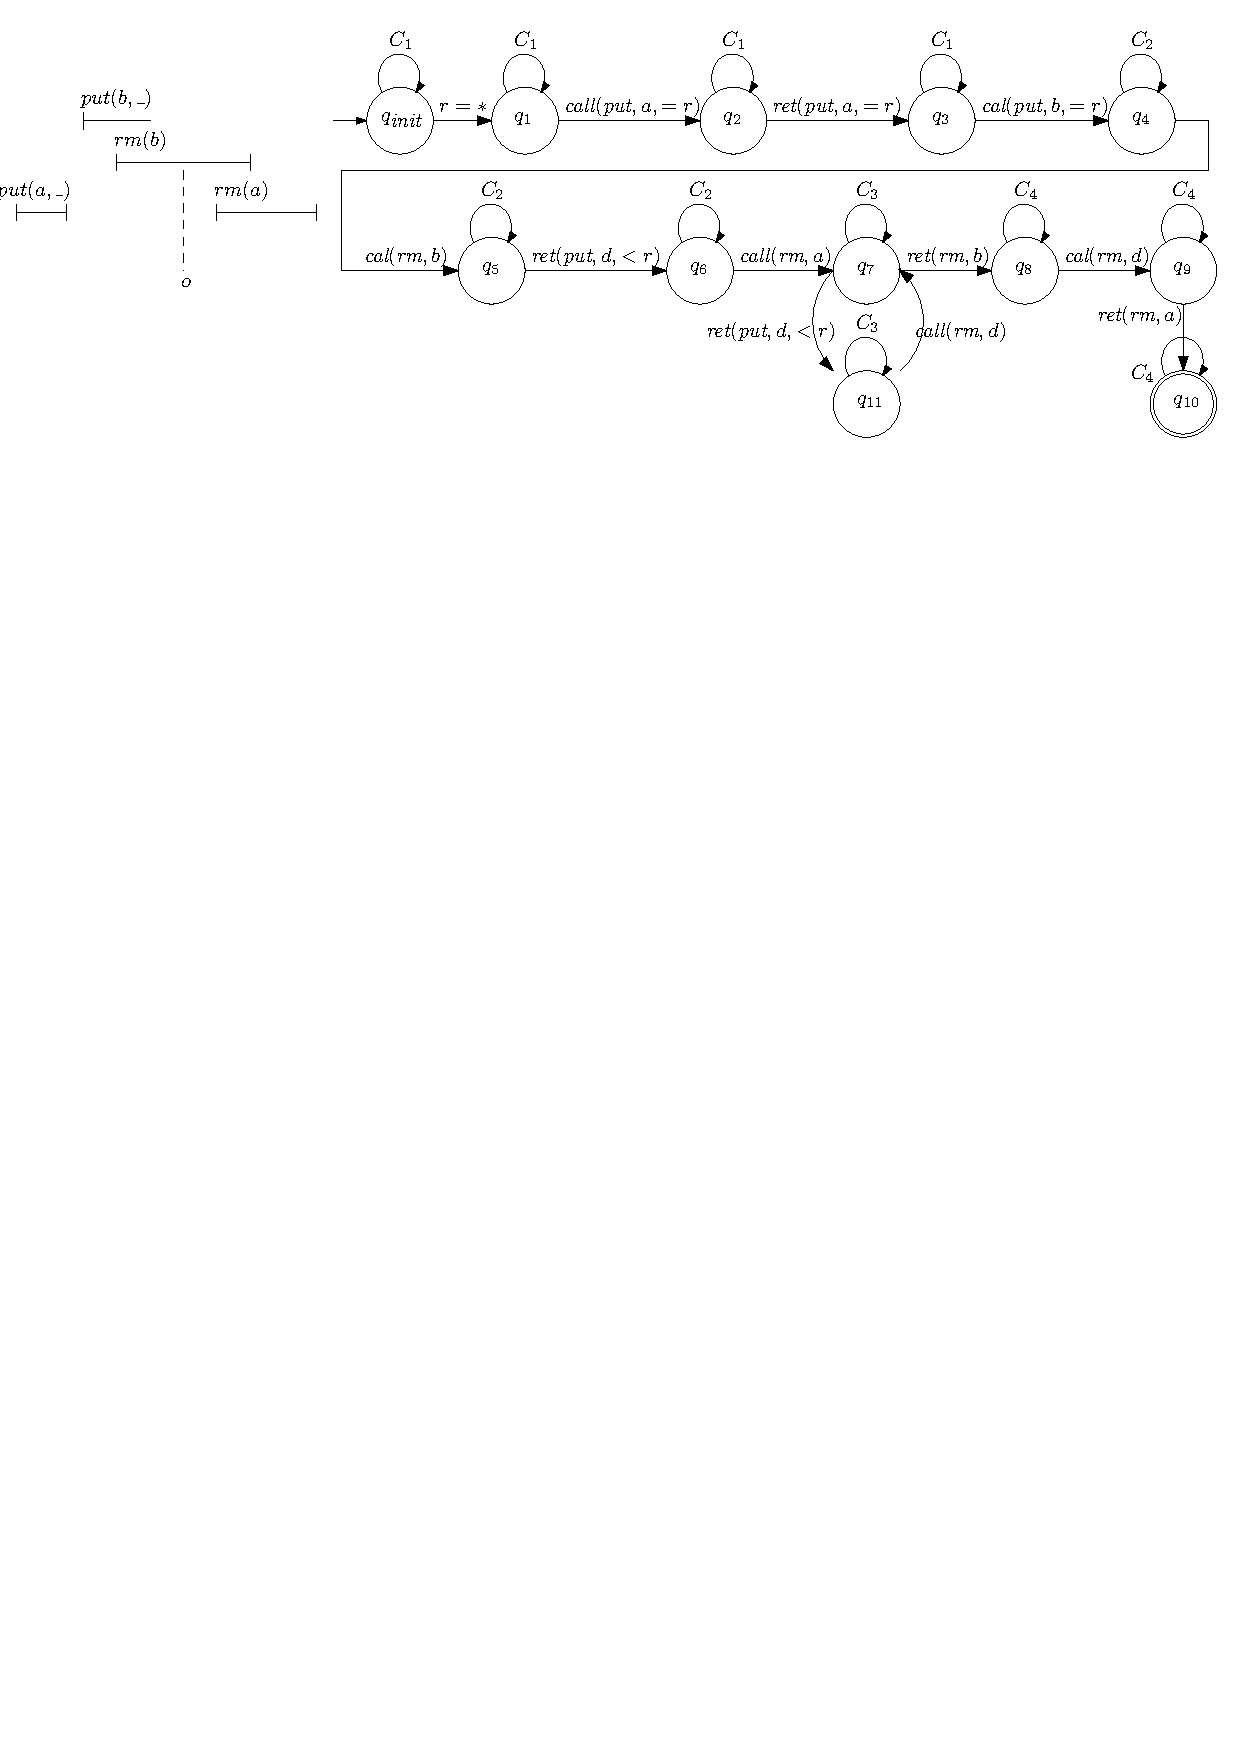
\includegraphics[width=0.8 \textwidth]{figures/PIC-Enumeration-WitnessAutomata.pdf}
%\vspace{-10pt}
  \caption{An enumerations and its witness automaton}
  \label{fig:an enumeration and its witness automaton}
\end{figure}


\subsection{Combine Step-by-Step linearizability and Co-Regular}
\label{subsec:combine step-by-step linearizability and co-regular}

We also prove that $\textit{EPQ}_2^{>}$, $\textit{EPQ}_2^{=}$ and $\textit{EPQ}_3$ are co-regular in Appendix \ref{subsec:appendix co-regular of EPQ2Lar}, Appendix \ref{subsec:appendix co-regular of EPQ2Equal} and Appendix \ref{subsec:co-regular of EPQ3}, respectively. Then we can see that $\textit{EPQ}$ is co-regular.

\begin{restatable}{lemma}{EPQIsCoRegular}
\label{lemma:EPQ is co-regular}
$\textit{EPQ}$ is co-regular.
\end{restatable}

By Lemma \ref{lemma:EPQ as multi in MRpri for history} and Lemma \ref{lemma:EPQ is co-regular}, we can finally reduce the verification of linearizability w.r.t $\textit{EPQ}$ into a reachability problem, as illustrated by the following theorem, where $\textit{Auts}_{\textit{EPQ}}$ is the set of witness automata of this section.

\begin{restatable}{theorem}{ReduceEPQIntoStateReachability}
\label{lemma:reduce EPQ into state reachability}
Given a data-independence implementation $\mathcal{I}$. $\mathcal{I} \sqsubseteq \textit{EPQ}$, if and only if, $\mathcal{I} \cap \textit{Auts}_{\textit{EPQ}} = \emptyset$.
\end{restatable}



